% !TEX encoding = UTF-8
\documentclass[fontsize=12pt,paper=letter,twoside]{scrartcl}
% Various imports and themes
\usepackage[top=4cm,bottom=4cm,left=3cm,right=3cm,asymmetric]{geometry}
%\geometry{landscape}
  % Activate for for rotated page geometry
%\usepackage[parfill]{parskip}    
  % Begin paragraphs with an empty line rather than an indent
\usepackage[table,xcdraw]{xcolor}
\usepackage{graphicx}

\usepackage{amsmath}
\usepackage{amssymb}
\usepackage{epstopdf}
\DeclareGraphicsRule{.tif}{png}{.png}{`convert #1 `dirname #1`/`basename #1 .tif`.png}
% Listings needs package courier
\usepackage{listings} % Needs 
\usepackage{courier}

\usepackage[framemethod=TikZ]{mdframed}
\usepackage{url}

\usepackage{sty/bsymb} %% Event-B symbols
\usepackage{sty/eventB} %% REQ and ENV
\usepackage{sty/calculation}
\usepackage{sty/mathpartir}

% \usepackage{sty/tikz-uml}


%Maths
\usepackage{amssymb,amsmath}
\def\Fl{\mathbb{F}}
\def\Rl{\mathbb{R}}
\def\Nl{\mathbb{N}}
\def\Bl{\mathbb{B}}
\def\St{\mathbb{S}}
\newcommand{\ovr}{\upharpoonright}
\newcommand{\var}[1]{\textit{#1}}
%Useful definitions
\newcommand{\mv}[1]{\textit{m\_#1}}
\newcommand{\cv}[1]{\textit{c\_#1}}
\newcommand{\degree}[1]{^{\circ}\mathrm{#1}}
%\newcommand{\comment}[1]{{\footnotesize \quad\texttt{--}\textrm{#1}}}
\newcommand{\im}[1]{i\texttt{-\!#1}}

\usepackage[headsepline]{scrpage2}
\pagestyle{scrheadings}
\ihead[]{\small EECS4312 Report1}
\ohead[]{\small \thepage}
\cfoot[]{}
\ofoot[]{}


%%%%PVS environment%%%%%%%%%%%%%%%%%%%
\lstnewenvironment{pvs}[1][]
    {\lstset{#1,captionpos=b,language=pvs,
    mathescape=true,
    basicstyle=\small\ttfamily,
    numbers=none,
    frame=single,
    % numberstyle=\tiny\color{gray},
    % backgroundcolor=\color{lightgray},
    firstnumber=auto
    }}
    {}
 %%%%%%%%%%%%%%%%%%%%%%%%%%%%%%%%
 
%%%%PVS environment%%%%%%%%%%%%%%%%%%%
\lstnewenvironment{events}[1][]
    {\lstset{#1,captionpos=b,language=events,
    mathescape=true,
    basicstyle=\small\ttfamily,
    numbers=none,
    frame=single,
    % numberstyle=\tiny\color{gray},
    % backgroundcolor=\color{lightgray},
    firstnumber=auto
    }}
    {}
 %%%%%%%%%%%%%%%%%%%%%%%%%%%%%%%%
 
%%%%Verbatim environment%%%%%%%%%%%%%%%%%%%
\lstnewenvironment{code}[1][]
    {\lstset{#1,captionpos=b,
    mathescape=true,
    basicstyle=\scriptsize\ttfamily,
    numbers=none,
    frame=single,
    comment=[l][\color{red}]{--},
    % keywords = [1]{"->"},
    % numberstyle=\tiny\color{gray},
    % backgroundcolor=\color{lightgray},
    firstnumber=auto
    }}
    {}

% \newenvironment{boxed}[1]
%    {\begin{center}
%    #1\\[1ex]
%    \begin{tabular}{|p{0.9\textwidth}|}
%    \hline\\
%    }
%    { 
%    \\\\\hline
%    \end{tabular} 
%    \end{center}
%    }
 %%%%%%%%%%%%%%%%%%%%%%%%%%%%%%%%
 
 %Text in a box
\newenvironment{textbox}
    {\begin{center}
    \begin{tabular}{|p{0.9\textwidth}|}
    \hline\\
    }
    { 
    \\\\\hline
    \end{tabular} 
    \end{center}
    }

\usepackage{hyperref}

%Highlight \hl{}
\usepackage{soul}

\usepackage{enumitem}
\newlist{mylist}{itemize}{1}
\setlist[mylist]{label=\textbullet,leftmargin=1cm,nosep}

\usepackage{multirow}

% Reduce space between figure and caption
%\usepackage{caption}
%\captionsetup[table]{font=small,skip=0pt}     %% Adjust here
%or equivalently 
\usepackage[font=small,skip=4pt]{caption}

% Indent equations
%\setlength{\mathindent}{1cm}

% Set the header

%\afterpage{\clearpage}
\usepackage{afterpage}
\usepackage{fancyvrb}

% Allow better table placement?
\renewcommand\floatpagefraction{.9}
\renewcommand\topfraction{.9}
\renewcommand\bottomfraction{.9}
\renewcommand\textfraction{.1}   
\setcounter{totalnumber}{50}
\setcounter{topnumber}{50}
\setcounter{bottomnumber}{50}
\usepackage{morefloats}
\usepackage[section]{placeins}

\newcommand{\pre}[1]{{#1}_{-1}}
\newtheorem{defn}{Definition}%[section]
\newtheorem{lemma}{Lemma}%[section]
\newtheorem{theorem}{Theorem}%[section]

%Sequents
\usepackage{bussproofs}

% Hide sections
\newif\ifhideproofs
%\hideproofstrue %uncomment to hide proofs

% Needed for TLA
% \input{tla/tla-style.tex} % style file for TLA
% Reduce space around equations
\setlength{\abovedisplayskip}{3pt}
\setlength{\belowdisplayskip}{3pt}


 
\usepackage{pdfpages}
%%%%%%%%%%%%%%%%%%%%%%%%%%%%%%%%%%%%%%%%%%%%%%%%%%%%%%%%%%%%%%%%%%%%%%%%%
\begin{document}
%%%%%%%%%%%%%%%%%%%%%%%%%%%%%%%%%%%%%%%%%%%%%%%%%%%%%%%%%%%%%%%%%%%%%%%%%
% Title and Authors
\newcommand{\mytitle}{
	EECS2311-W20 Project:\\ Venn Create
}
\ihead[]{\small \mytitle}
\title{\mytitle}
\author{
	Chidalu Agbakwa (216337784) \and
	Jihal Patel (216376436) 	\and
	Shangru Li (214488993) 		\and
	Robert Suwary (215446016)
}
% Display a given date or no date
\date{\today}
\maketitle
%%%%%%%%%%%%%%%%%%%%%%%%%%%%%%%%%%%%%%%%%%%%%%%%%%%%%%%%%%%%%%%%%%%%%%%%%
\subsection*{Revisions}
\begin{tabular}{|l|l|p{3in}|}
	\hline
	Date & Revision& Description \\ 
	\hline
	08 February 2020 
	& 1.0       
	& Initial release of this document\\ 
	\hline
\end{tabular}
\bigskip\bigskip
%%%%%%%%%%%%%%%%%%%%%%%%%%%%%%%%%%%%%%%%%%%%%%%%%%%%%%%%%%%%%%%%%%%%%%%%%
\newpage
\vspace*{2in}
\begin{center}
	\huge{\textbf{User Manual}:\\ Venn Create}
\end{center}
\newpage
%%%%%%%%%%%%%%%%%%%%%%%%%%%%%%%%%%%%%%%%%%%%%%%%%%%%%%%%%%%%%%%%%%%%%%%%%
\newpage
\tableofcontents
\newpage
\listoffigures
\listoftables
%%%%%%%%%%%%%%%%%%%%%%%%%%%%%%%%%%%%%%%%%%%%%%%%%%%%%%%%%%%%%%%%%%%%%%%%%
\newpage
\section{Introduction}
Welcome to Venn Create - a desktop application that can draw customizable
Venn diagrams.

Venn Create enables user to easily create Venn diagrams with customized
labels, in different size and shape. Which can be used to compare and
contrast two or more objects, events, people, or concepts. Clearly
illustrating the differences and similarities between different entities
and all of this, with ZERO cost.

Venn Create provides a user-friendly interface, so that new users will
be able to use the application with minimum efforts. In addition,
the application provides essential functionalities, such as export/import
existing Venn diagrams, printing and customized theming.

%%%%%%%%%%%%%%%%%%%%%%%%%%%%%%%%%%%%%%%%%%%%%%%%%%%%%%%%%%%%%%%%%%%%%%%%%
\newpage
\section{Get Started}

\begin{figure}[hbt]
	\begin{mdframed}
		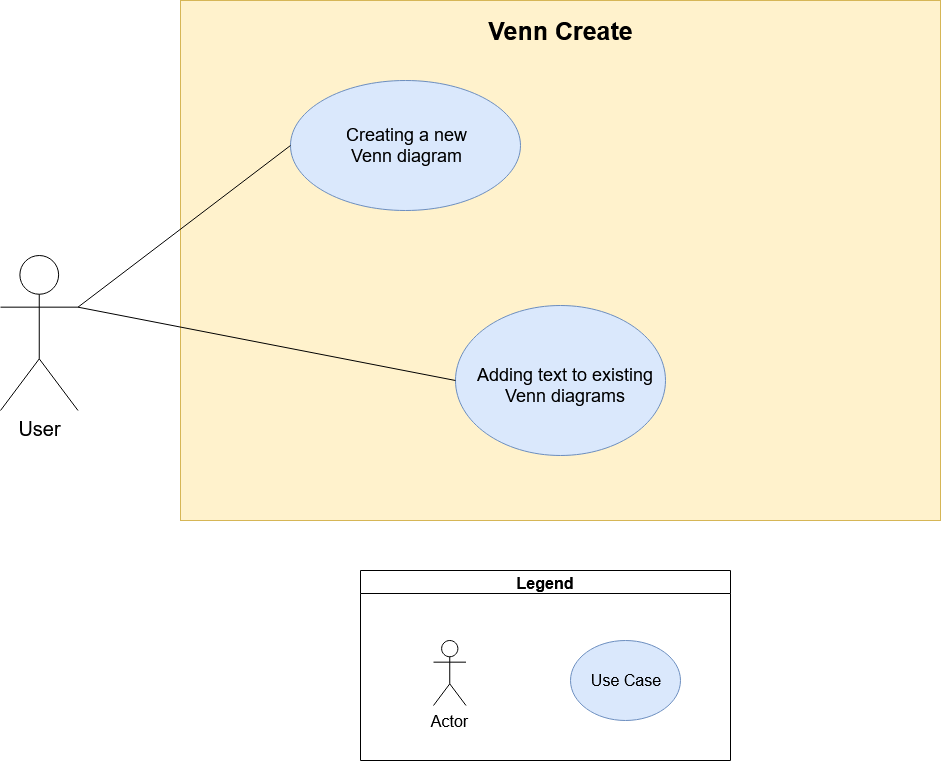
\includegraphics[width=\textwidth]{images/use-case-diagram.png}
	\end{mdframed}
	\caption{Use Case Diagram}
\end{figure}

%%%%%%%%%%%%%%%%%%%%%%%%%%%%%%%%%%%%%%%%%%%%%%%%%%%%%%%%%%%%%%%%%%%%%%%%%

\newpage
\section{Use Case Diagram and Textual Use Cases}



\newpage

\subsection*{Use Case Textual Description 1}

\begin{table}[h]
	\begin{tabular}{|l|}
		\hline
		\\
		Use case at1: Adding a Venn Diagram													\\
		\\
		This use case describes the operation of a user adding a new Venn diagram 			\\
		to the application. 																\\
		\\
		\underline{Related System Goals}: G1												\\
		\\
		\underline{Primary Actor}: User														\\
		\\
		\underline{Precondition}:															\\ \qquad
		User have already opened the application. 											\\
		\\
		\underline{Postcondition}:															\\ \qquad
		A new Venn diagram has been added to the application.								\\
		\\
		\underline{Main success scenario}:													\\
		\begin{minipage}{6in}
			\vskip 4pt
			\begin{enumerate}
				\item The user may view the existing Venn diagrams displayed on the application
						(if there is any), and familiarize themselves with the user interface
						of the program.
				\item When ready the user will add a new Venn diagram to the application.
			\end{enumerate}
			\vskip 4pt
		\end{minipage}
		\\
		\hline
	\end{tabular}
\end{table}

\newpage

\subsection*{Use Case Textual Description 2}

\begin{table}[h]
	\begin{tabular}{|l|}
		\hline
		\\
		Use case at2: Adding text label to existing Venn diagrams.							\\
		\\
		Given that at least one Venn diagram exists in the application, this use case		\\
		describes how a user add a text label to an existing Venn diagram.					\\
		\\
		\underline{Related System Goals}: G1												\\
		\\
		\underline{Primary Actor}: User														\\
		\\
		\underline{Precondition}:															\\ \qquad
		At least one Venn diagram exists in the application.								\\
		\\
		\underline{Postcondition}:															\\ \qquad
		A text label is added to an existing Venn diagram.									\\
		\\
		\underline{Main success scenario}:													\\
		\begin{minipage}{6in}
			\vskip 4pt
			\begin{enumerate}
				\item User chooses which Venn diagram to add the new text label.
				\item User type in the content of the new text label to be added.
				\item The text label is added to the corresponding Venn diagram.
			\end{enumerate}
			\vskip 4pt
		\end{minipage}
		\\
		\hline
	\end{tabular}
\end{table}

%%%%%%%%%%%%%%%%%%%%%%%%%%%%%%%%%%%%%%%%%%%%%%%%%%%%%%%%%%%%%%%%%%%%%%%%%
\newpage
\section{E-Descriptions: Environmental Constraints}

\reqm{ENV}{The application will run on desktop computers.\\}
{Traceability reference: see Purpose.}

%%%%%%%%%%%%%%%%%%%%%%%%%%%%%%%%%%%%%%%%%%%%%%%%%%%%%%%%%%%%%%%%%%%%%%%%%
\newpage

\section{R-Descriptions: Functional Requirements}

\reqm{REQ}{User shall be able to add new Venn diagrams to the application.\\}
{Traceability reference: see High level goals, Purpose and acceptance test at1.}

\reqm{REQ}{User shall be able to add text labels to the existing Venn diagrams.\\}
{Traceability reference: see High level goals, Purpose and acceptance test at2.}

%%%%%%%%%%%%%%%%%%%%%%%%%%%%%%%%%%%%%%%%%%%%%%%%%%%%%%%%%%%%%%%%%%%%%%%%%
\newpage
\section{User Interface}

This is the user interface of Venn create.

\begin{figure}[hbt]
	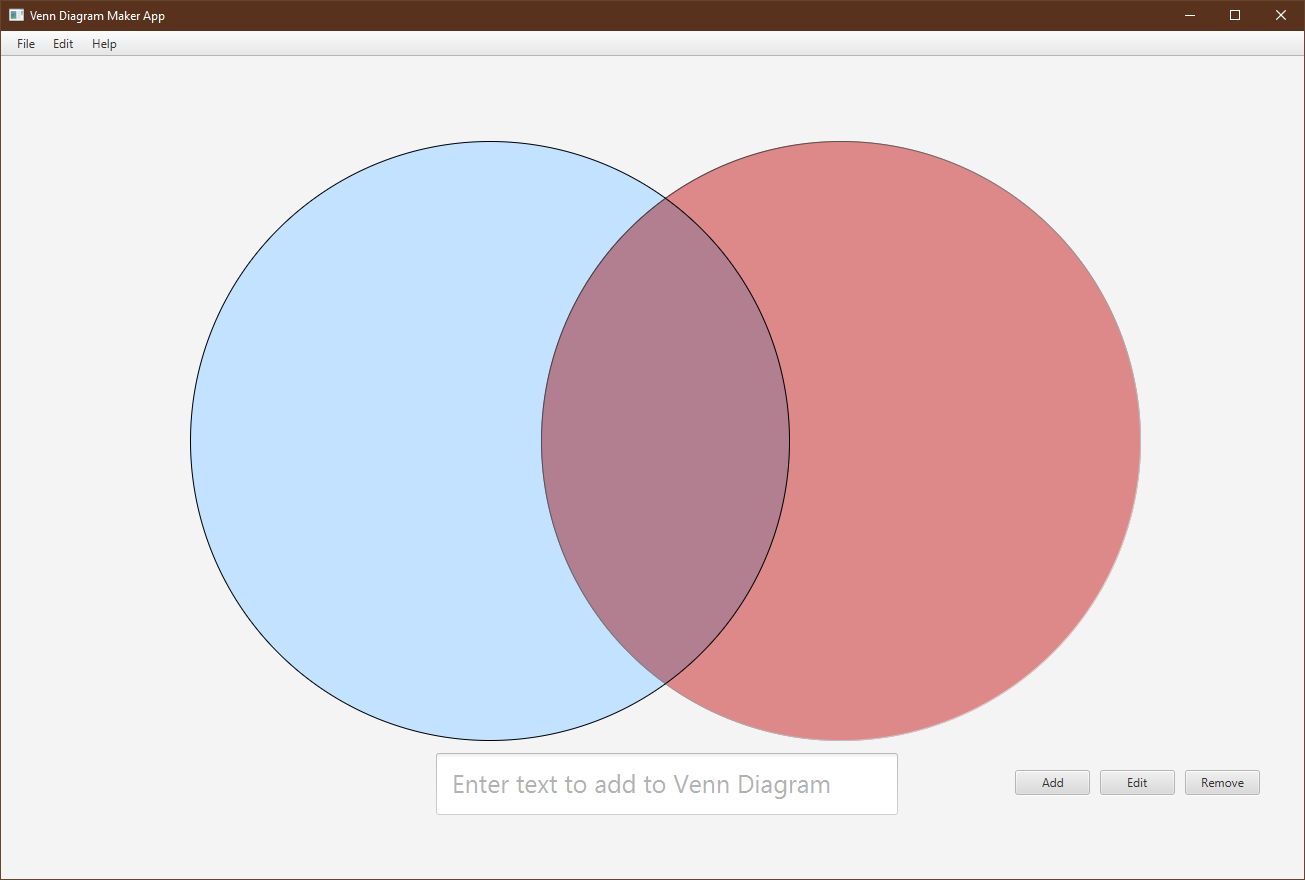
\includegraphics[width=\textwidth]{images/user-interface.png}
	\caption{User Interface of Venn Create}
\end{figure}

%%%%%%%%%%%%%%%%%%%%%%%%%%%%%%%%%%%%%%%%%%%%%%%%%%%%%%%%%%%%%%%%%%%%%%%%
\newpage
\section{Acceptance Tests}

The table below describes the relationship between our use cases and concrete acceptance tests.

\begin{table}[!ht]
	\centering
	\begin{tabular}{|l|l|l|}
		\hline
		\multicolumn{1}{|c|}{\textbf{Use Cases}} & \multicolumn{1}{c|}{\textbf{Description}}                                    & \multicolumn{1}{c|}{\textbf{Acceptance Tests}} \\ \hline
		UC1                                      & Adding a Venn diagram                  & at1                                            \\ \hline
		UC2                                      & Adding a text label to existing Venn diagrams.                        			     & at2                                            \\ \hline
	\end{tabular}
	\caption{Acceptance Tests for each Use Case}
	\label{acceptance-tests}
\end{table}

The following pages contain detailed descriptions of acceptance tests at1-at2.

\begin{table}[!h]
	\begin{tabular}{|l|}
		\hline
		\\
		\textbf{\emph{Acceptance Test at1}} 	
		\\\\
		\underline{Purpose}: Testing the add Venn digram functionality						\\
		\\
		\underline{Category}: Basic															\\
		\\
		\underline{Precondition}:															\\ \qquad
		User has successfully opened the application.										\\
		\\
		\underline{Reproduction Steps:}
		\\ \qquad 1. In the menu bar, click 'File'.
		\\ \qquad \textit{Result: A menu bar drop down menu is displayed. }
		\\\\ \qquad 2. In the drop down menu, click 'Add Venn diagram'.
		\\ \qquad \textit{Result: A new Venn diagram is added and displayed on the application.}
		\\\\
		\hline
	\end{tabular}
\end{table}

\newpage

\begin{table}[!h]
	\begin{tabular}{|l|}
		\hline
		\\
		\textbf{\emph{Acceptance Test at2}} 	
		\\\\
		\underline{Purpose}: Testing the add text label to existing Venn diagram functionality \\
		\\
		\underline{Category}: Basic		\\
		\\
		\underline{Precondition}:															\\ \qquad
		User has successfully opened the application.
		\\ \qquad
		At least one Venn diagram exists in the application.
		\\\\
		\underline{Reproduction Steps}:				
		\\\\ \qquad 1. Click the text field at the lower centre of the application.
		\\ \qquad \textit{Result: Text field should be ready to accept user input.} 
		\\\\ \qquad 2. Type 'Foo' to the text field.
		\\ \qquad \textit{Result: Text field should now display 'Foo'.} 
		\\\\ \qquad 3. Click the 'Add' button on the right side of the text field.
		\\ \qquad \textit{Result: A text label contains 'Foo' is added to Venn Diagram.} 
		\\\\
		\hline
	\end{tabular}
\end{table}

%%%%%%%%%%%%%%%%%%%%%%%%%%%%%%%%%%%%%%%%%%%%%%%%%%%%%%%%%%%%%%%%%%%%%%%%
\newpage
\section{Traceability Matrix}

The following table outlines which R-descriptions are tested by which acceptance tests.

\begin{table}[!ht]
	\centering
	\begin{tabular}{|l|l|l|l|l|l|l|l|}
		\hline
		\textbf{REQ} & at1 & at2 \\ \hline
		REQ2         & X   &     \\ \hline
		REQ3         &     & X   \\ \hline
	\end{tabular}
	\caption{Traceability matrix for R-descriptions}
	\label{tbl:at}
\end{table}

%%%%%%%%%%%%%%%%%%%%%%%%%%%%%%%%%%%%%%%%%%%%%%%%%%%%%%%%%%%%%%%%%
\end{document} 	

